\chapter{Výsledky}
Pro zhodnocení výsledků našeho vyhledávače jsme provedli dva druhy testů. V
rámci prvního jsme porovnávali výsledky našeho vyhledávače s ostatními veřejně
dostupnými vyhledávači spojení. V druhém testu jsme na pevně dané trase a času
zkoumali, jaký vliv na nalezené trasy má různé nastavení penalt a rychlostí
chůze. Aplikaci jsme také profilovali, abychom zjistili, v jakých částech se
tráví nejvíce času a měly by se optimalizovat jako první.

\section{Porovnání s jinými vyhledávači}
Výsledky našeho vyhledávače jsme porovnávali s veřejně dostupnými vyhledávači
spojení po Praze: IDOS\footnote{\url{http://idos.cz}},
Mapy.cz\footnote{\url{http://mapy.cz}} a Google
Maps\footnote{\url{http://maps.google.com}}. 

IDOS je nejstarší a nejznámější vyhledávač spojení. Jako jediný z vyhledávačů
nepodporuje hledání pěších tras, vyhledává pouze v jízdních řádech, přestupy
mezi zastávkami řeší pomocí tabulky, která obsahuje dvojice zastávek a čas
přesunu mezi nimi. Jako vstup je možné zadat adresu, ale vyhledávač nalezne
pouze nejbližší zastávky podle vzdušné vzdálenosti a hledá z nich / do nich. 
Na druhou stranu umožňuje široké možnosti nastavení vyhledávání spojů -- volbu
minimálních časů na přestup, typů dopravních prostředků, počtu přestupů, \dots

Mapy.cz a Google Maps jsou původně mapové služby, které do svých vyhledávačů
přidaly možnost vyhledávání kromě pěších cest i spojení MHD. Protože se jedná
primárně o mapové služby, vyhledávače neumožňují žádné (Mapy.cz) nebo jen velmi
omezené (Google Maps) přizpůsobení. 

Při porovnávání vyhledaných spojení jsme všude nechali výchozí nastavení a náš
vyhledávač jsme nastavili tak, jak si myslíme, že jsou nastaveny ostatní
vyhledávače, aby byly výsledky porovnatelné. Konkrétní nastavení je výchozí
nastavení {\tt config/speeds.yaml} v příloze. Přestupy nebyly nijak
penalizovány, na zastávce bylo nutné mít aspoň 30\,s čas mezi příchodem /
příjezdem a odjezdem.

Testovali jsme následující trasy, které známe i z reálného provozu. Jednotlivé
trasy zkoumaly různé aspekty vyhledávačů:
\begin{itemize}
	\item {\em Kolej 17. listopadu -- Přírodovědecká fakulta UK, Albertov}\\ Tato
	cesta je zaměřena na obtížnou dopravní situaci okolo kolejí 17.
	listopadu. Spojení na Nádraží Holešovice je nejspolehlivější pěšky,
	autobus 201 většinou nejede dle jízdního řádu. V případě cesty tramvají
	č. 17 je možné jednak využít od kolejí autobus 112, ovšem s výstupem na
	Povltavské, nikoli na Trojské, případně dojít přímo na Trojskou pěšky.
	Všechny tyto možnosti dávají smysl při hledání cesty na Albertov. Na
	durhém konci také není situace přímočará, při cestě od metra je dobrou
	alternativou jít pěšky z Vyšehradu. 
	\item {\em Kolej 17. listopadu -- Čistírna odpadních vod, Bubeneč}\\ Tato
	cesta zkoumá schopnosti pěší navigace, protože jednou z možností je jít
	pěšky přes Stromovku. Také je zde vidět rozdíl mezi naším vyhledávačem a
	Google Maps na jedné straně a IDOSem a Mapy.cz na straně druhé, které
	využívají znalosti jízdních řádů integrovaných vlaků a umí je na této
	cestě využít.
	\item {\em Kovanecká -- Gymnázium Omská}\\ Tato cesta opět zkoumá schopnost
	využívat delší pěší přesuny a také dávat přednost časově kratším cestám
	s přestupy. 
	\item {\em FEL ČVUT, Dejvice -- Hlávkova kolej}\\ Tato cesta je zaměřena na
	hledání aktuálně nejrychlejší alternativy z několika rovnocenných. Dobré
	alternativy nevyžadují dlouhé pěší přesuny.
\end{itemize}
\subsection{Kolej 17.\,listopadu -- Albertov}

Náš vyhledávač našel následující spojení:

Spojení 0:\\[2mm]
\begin{tabular}{|l|c|c|r|}\hline
{\bf Zastávka}&{\bf Příjezd}&{\bf Odjezd}&{\bf Linka}\\\hline
Kuchyňka&&13:25&201\\\hline
Nádraží Holešovice&13:28&13:32&C\\\hline
I. P. Pavlova&13:40&&\\\hline
\end{tabular} \\[2mm]
Očekávaný příchod je 13:56.

Spojení 2:\\[2mm]
\begin{tabular}{|l|c|c|r|}\hline
{\bf Zastávka}&{\bf Příjezd}&{\bf Odjezd}&{\bf Linka}\\\hline
Kuchyňka&&13:25&201\\\hline
Nádraží Holešovice&13:28&13:32&C\\\hline
Florenc&13:36&13:41&B\\\hline
Karlovo náměstí&13:46&&\\\hline
Palackého náměstí&&13:52&18\\\hline
Albertov&13:56&&\\\hline
\end{tabular} \\[2mm]
Očekávaný příchod je 14:00.

Spojení 3:\\[2mm]
\begin{tabular}{|l|c|c|r|}\hline
{\bf Zastávka}&{\bf Příjezd}&{\bf Odjezd}&{\bf Linka}\\\hline
Kuchyňka&&13:25&201\\\hline
Nádraží Holešovice&13:28&13:31&6\\\hline
Masarykovo nádraží&13:43&13:44&14\\\hline
Albertov&13:59&&\\\hline
\end{tabular}\\[2mm]
Očekávaný příchod je 14:03.

Vyhledávač IDOS našel následující spojení\\
\begin{tabular}{|l|c|c|r|}\hline
{\bf Zastávka}&{\bf Příjezd}&{\bf Odjezd}&{\bf Linka}\\\hline
Kuchyňka&&13:23&201\\\hline
Bulovka&13:26&13:28&24\\\hline
Albertov&14:04&&\\\hline
\end{tabular}\\
\begin{tabular}{|l|c|c|r|}\hline
{\bf Zastávka}&{\bf Příjezd}&{\bf Odjezd}&{\bf Linka}\\\hline
Kuchyňka&&13:25&201\\\hline
Nádraží Holešovice&13:28&13:32&C\\\hline
Florenc&13:36&13:41&B\\\hline
Karlovo náměstí&13:47&&\\\hline
Palackého náměstí&&13:52&18\\\hline
Albertov&13:56&&\\\hline
\end{tabular} 

V tomto spojení se ukázala výhoda vyhledávačů, které umí delší pěší přesuny.
Vlivem výluky není možné jet přímo z Karlova náměstí na Albertov a nejkratší
cesta se ukazuje být přes I. P. Pavlova. Náš vyhledávač našel tuto trasu ve
stejné podobě jako Google Maps, Mapy.cz ještě využily autobusu 148 k přiblížení
se. Odhadované časy se liší jen o rychlost chůze. IDOS kvůli absenci mapových
podkladů nalezl jen trasy vedoucí na Albertov, které náš vyhledávač nalezl také,
i když s mírně jiným průběhem. 

\begin{tabular}{|l|c|c|r|}\hline
{\bf Zastávka}&{\bf Příjezd}&{\bf Odjezd}&{\bf Linka}\\\hline
Pelc Tyrolka&&13:26&112\\\hline
Trojská&13:29&13:33&17\\\hline
Výtoň&13:54&13:57&14\\\hline
Albertov&13:59&&\\\hline
\end{tabular} 
\begin{figure}[h]
  \centering
    \includegraphics[scale=.5]{../img/kolej-albertov-standard.pdf}
  \caption{Spojení Kolej 17. listopadu -- Albertov podle našeho vyhledávače}
  \label{fig:kolej-albertov-osmawalk}
\end{figure}
\begin{figure}[h]
  \centering
    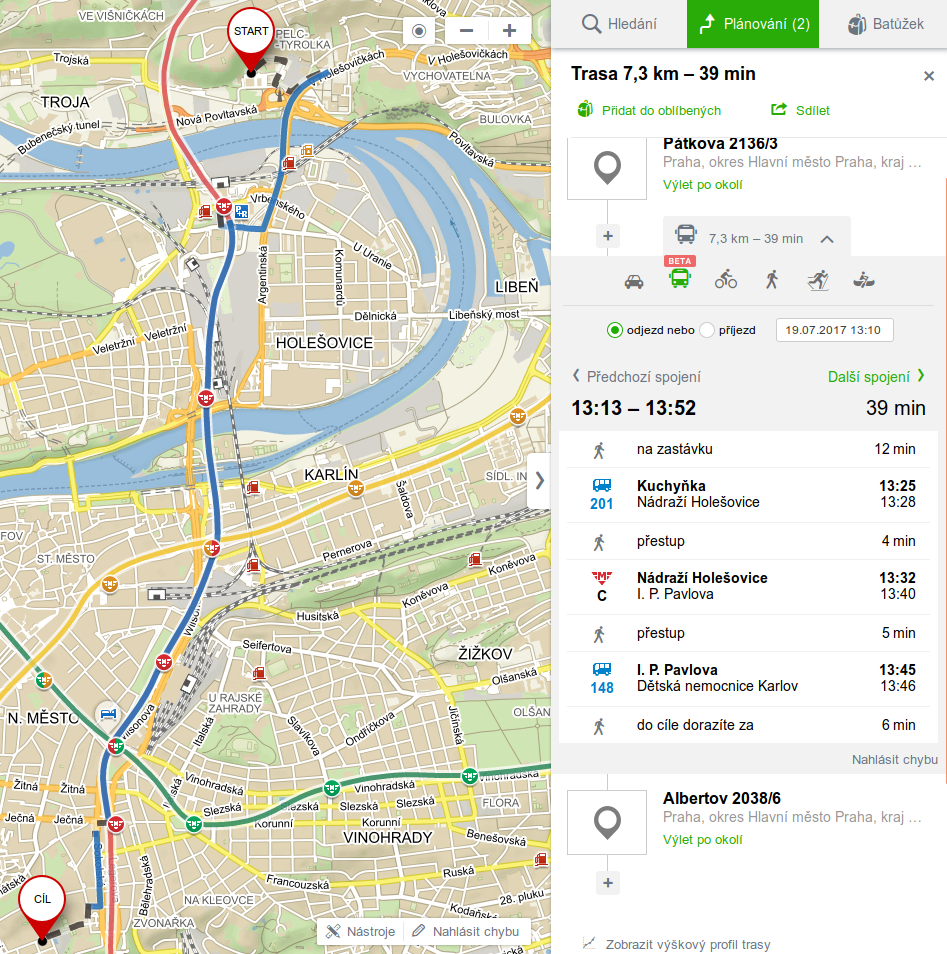
\includegraphics[width=\textwidth]{../img/kolej-albertov-seznam.png}
  \caption{Spojení Kolej 17. listopadu -- Albertov podle Mapy.cz}
  \label{fig:kolej-albertov-seznam}
\end{figure}
\begin{figure}[h]
  \centering
    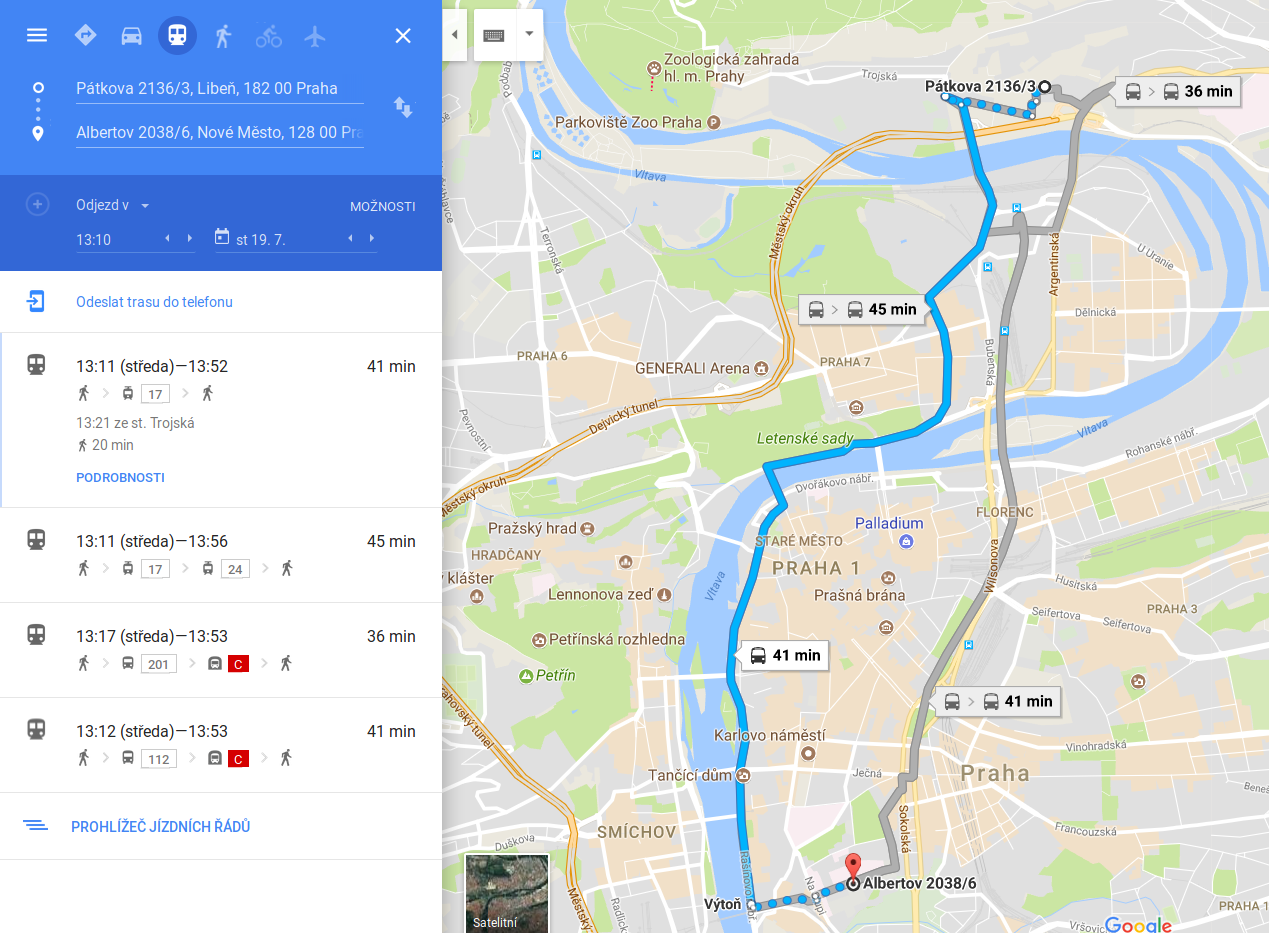
\includegraphics[width=\textwidth]{../img/kolej-albertov-google.png}
  \caption{Spojení Kolej 17. listopadu -- Albertov podle Google Maps}
  \label{fig:kolej-albertov-google}
\end{figure}

\clearpage
\subsection{Kolej 17.\,listopadu -- Čistírna odpadních vod}

Spojení 0 nevyžaduje žádný přesun pomocí MHD, celá trasa je vedena pěšky.
Očekávaný příchod je 14:08.

Spojení 1:\\[2mm]
\begin{tabular}{|l|c|c|r|}\hline
{\bf Zastávka}&{\bf Příjezd}&{\bf Odjezd}&{\bf Linka}\\\hline
Kuchyňka&&13:25&201\\\hline
Nádraží Holešovice&13:28&13:31&6\\\hline
Strossmayerovo náměstí&13:36&13:39&26\\\hline
Hradčanská&13:47&14:00&131\\\hline
Goeteho&14:03&&\\\hline
\end{tabular}\\[2mm]
Očekávaný příchod je 14:08.

Spojení 4:\\[2mm]
\begin{tabular}{|l|c|c|r|}\hline
{\bf Zastávka}&{\bf Příjezd}&{\bf Odjezd}&{\bf Linka}\\\hline
Kuchyňka&&13:25&201\\\hline
Nádraží Holešovice&13:28&13:31&6\\\hline
Strossmayerovo náměstí&13:36&13:39&26\\\hline
Vítězné náměstí&13:50&&\\\hline
Dejvická&&13:55&160\\\hline
Nádraží Podobaba&13:59&&\\\hline
\end{tabular}\\[2mm]
Očekávaný příchod je 14:09. 

Spojení 6:\\[2mm]
\begin{tabular}{|l|c|c|r|}\hline
{\bf Zastávka}&{\bf Příjezd}&{\bf Odjezd}&{\bf Linka}\\\hline
Kuchyňka&&13:25&201\\\hline
Nádraží Holešovice&13:28&13:31&6\\\hline
Dlouhá třída&13:38&13:42&8\\\hline
Nádraží Podbaba&14:02&&\\\hline
\end{tabular}\\[2mm]
Očekávaný příchod je 14:12. 


Vyhledávač IDOS našel následující spojení:\\
\begin{tabular}{|l|c|c|r|}\hline
{\bf Zastávka}&{\bf Příjezd}&{\bf Odjezd}&{\bf Linka}\\\hline
Kuchyňka&&13:25&201\\\hline
Nádraží Holešovice&13:28&13:45&Os 10440\\\hline
Praha-Podbaba&13:49&&\\\hline
\end{tabular}\\
\begin{tabular}{|l|c|c|r|}\hline
{\bf Zastávka}&{\bf Příjezd}&{\bf Odjezd}&{\bf Linka}\\\hline
Pelc Tyrolka&&13:26&112\\\hline
Trojská&13:29&13:33&17\\\hline
Nádraží Holešovice&13:35&13:45&Os 10440\\\hline
Praha-Podbaba&13:49&&\\\hline
\end{tabular} 

Na výsledcích tohoto spojení se významně projevila integrace železničních
jízdních řádů do vyhledávačů. IDOS i Mapy.cz jízdní řády integrované mají,
proto využily vlak mezi stanicemi Praha-Holešovice a Praha-Podbaba. Google Maps
ani náš vyhledávač železniční jízdní řády integrované nemají, nalezly proto
cesty oklikou a s delšími pěšími přesuny. Náš vyhledávač nalezl obě varianty
cesty bez vlaků, a to přímo pěšky a oklikou přes Letnou, pro přímou cestu při
tomto hledání nevyužil autobus 112 a proto je očekávaný čas horší než u Google
Maps. Jak se také ukáže u dalších spojení, odhad rychlosti chůze byl při našem
nastavení o něco konzervativnější než u Google Maps, vzálenější pěší přesuny
tudíž vycházejí o něco delší.


\begin{figure}[h]
  \centering
    \includegraphics[width=\textwidth]{../img/kolej-bubenec-osmawalk.pdf}
  \caption{Spojení Kolej 17. listopadu -- Čistírna odpadních vod podle našeho
  vyhledávače}
  \label{fig:kolej-bubenec-osmawalk}
\end{figure}
\begin{figure}[h]
  \centering
    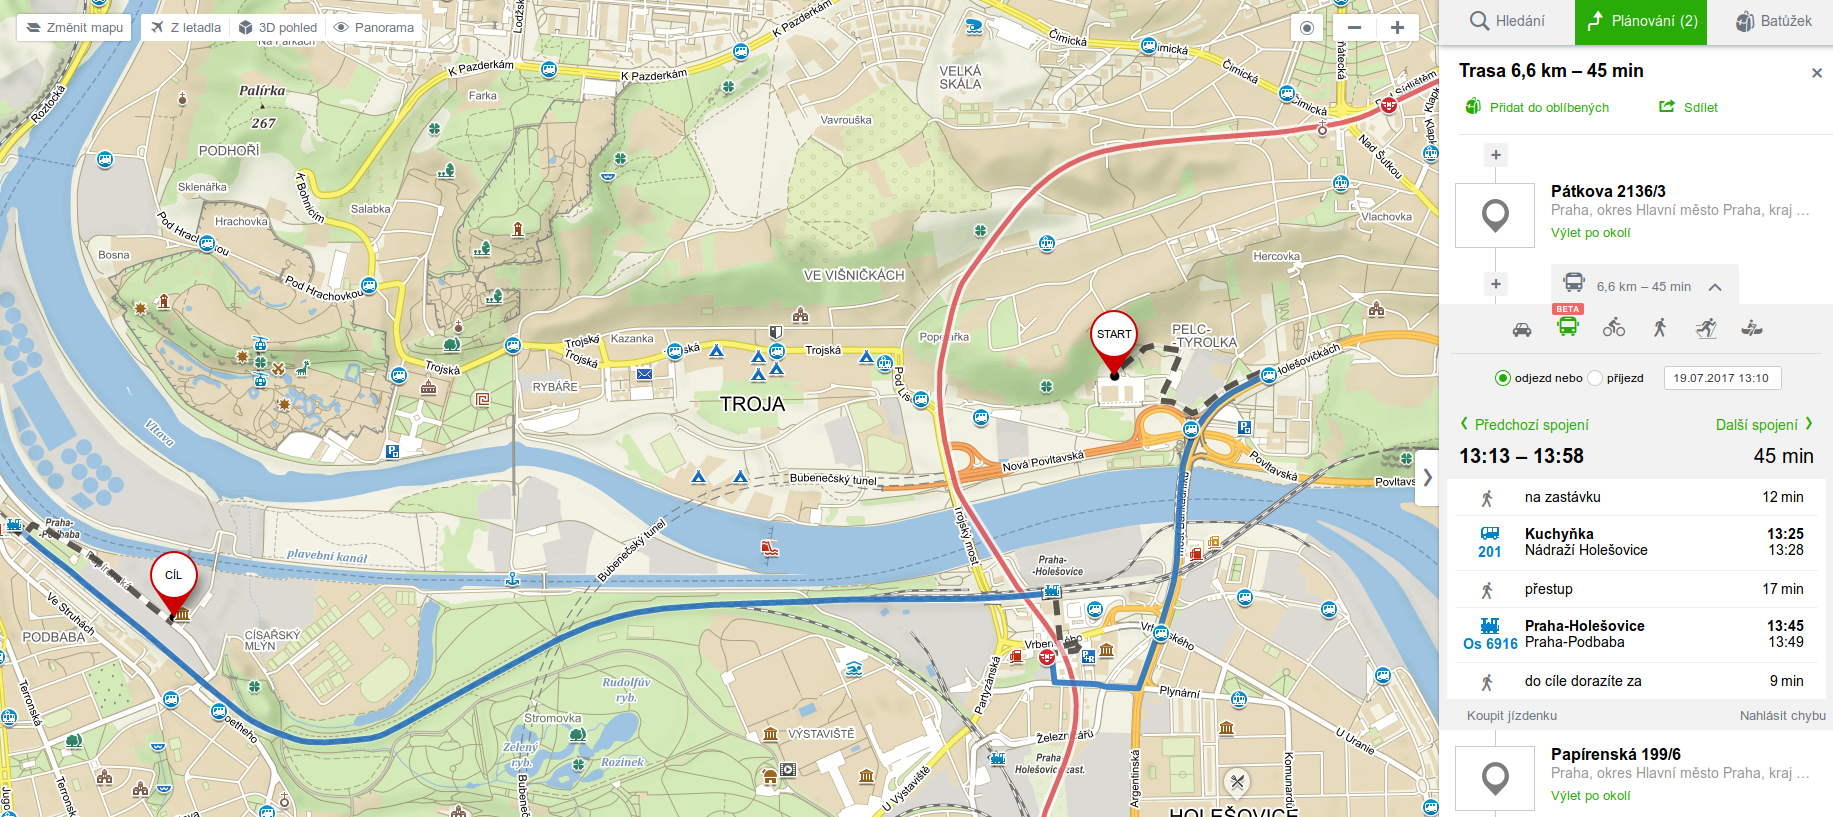
\includegraphics[width=\textwidth]{../img/kolej-bubenec-seznam.png}
  \caption{Spojení Kolej 17. listopadu -- Čistírna odpadních vod podle Mapy.cz}
  \label{fig:kolej-bubenec-seznam}
\end{figure}
\begin{figure}[h]
  \centering
    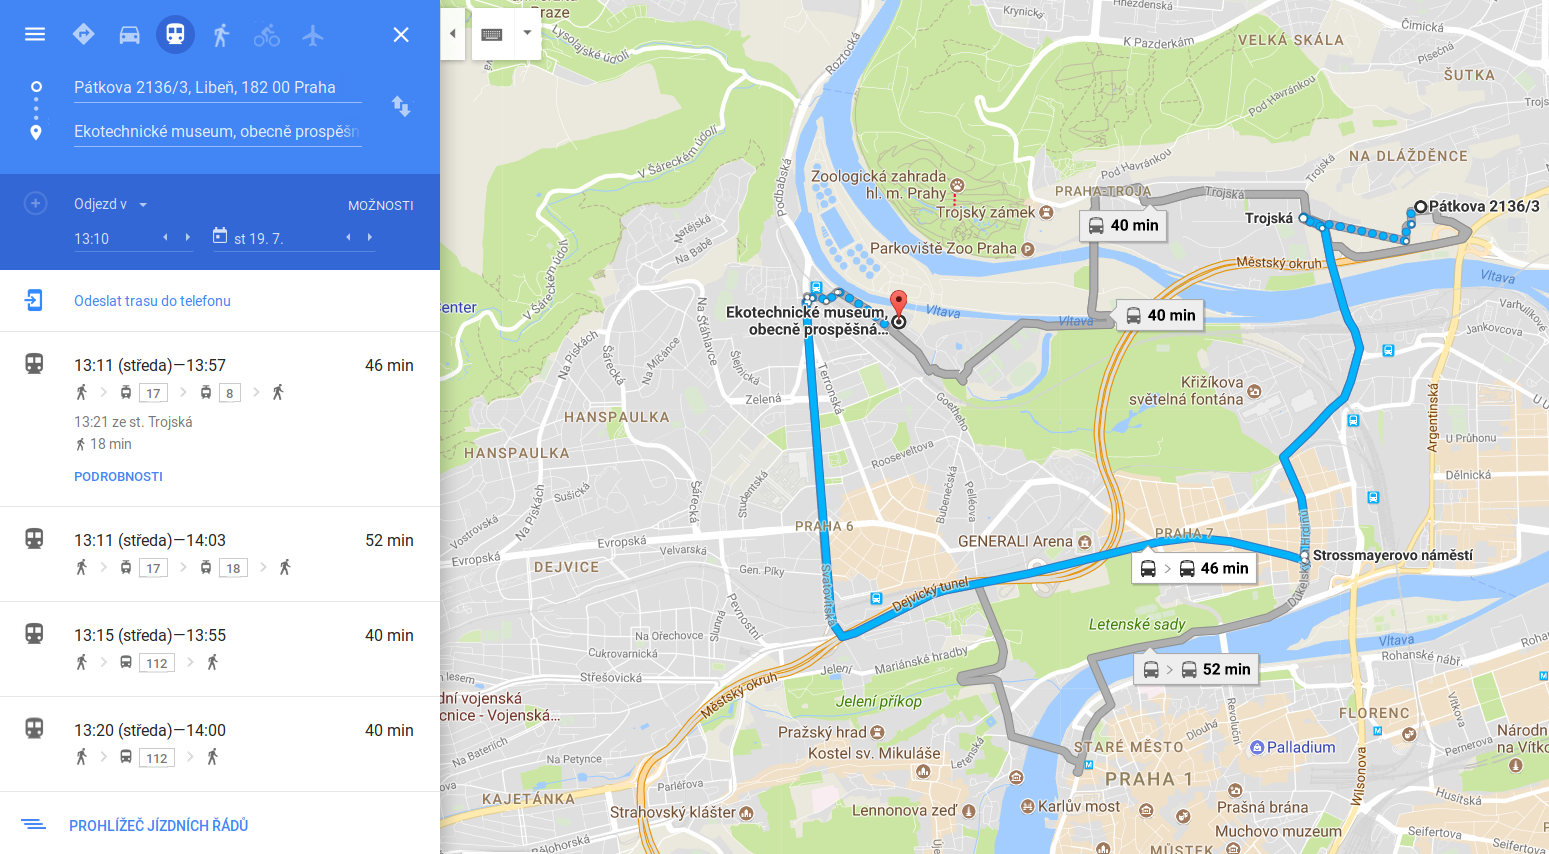
\includegraphics[width=\textwidth]{../img/kolej-bubenec-google.png}
  \caption{Spojení Kolej 17. listopadu -- Čistírna odpadních vod podle Google
  Maps}
  \label{fig:kolej-bubenec-google}
\end{figure}

\clearpage
\subsection{Kovanecká -- Gymnázium Omská}
Spojení 0:\\[2mm]
\begin{tabular}{|l|c|c|r|}\hline
{\bf Zastávka}&{\bf Příjezd}&{\bf Odjezd}&{\bf Linka}\\\hline
Divadlo Gong&&13:21&16\\\hline
Orionka&13:39&13:41&136\\\hline
Bělocerkevská&13:47&&\\\hline
\end{tabular}\\[2mm]
Očekávaný příchod je 13:55.
 
Spojení 1:\\[2mm]
\begin{tabular}{|l|c|c|r|}\hline
{\bf Zastávka}&{\bf Příjezd}&{\bf Odjezd}&{\bf Linka}\\\hline
Divadlo Gong&&13:21&16\\\hline
Mezi hřbitovy&13:32&13:36&26\\\hline
Nad Primaskou&13:42&13:43&7\\\hline
Slavia&13:49&13:52&22\\\hline
Kubánské náměstí&13:53&&\\\hline
\end{tabular}\\[2mm]
Očekávaný příchod je 13:55.
 

Spojení 3:\\[2mm]
\begin{tabular}{|l|c|c|r|}\hline
{\bf Zastávka}&{\bf Příjezd}&{\bf Odjezd}&{\bf Linka}\\\hline
Balabenka&&13:19&25\\\hline
Palmovka&13:21&13:23&24\\\hline
Karlovo náměstí&13:45&13:46&22\\\hline
Kubánské náměstí&14:05&&\\\hline
\end{tabular}\\[2mm]
Očekávaný příchod je 14:07.
 
Spojení 5:\\[2mm]
\begin{tabular}{|l|c|c|r|}\hline
{\bf Zastávka}&{\bf Příjezd}&{\bf Odjezd}&{\bf Linka}\\\hline
Balabenka&&13:19&25\\\hline
Palmovka&13:21&13:23&24\\\hline
Kubánské náměstí&14:06&&\\\hline
\end{tabular}\\[2mm]
Očekávaný příchod je 14:08.
 
Spojení 7:\\[2mm]
\begin{tabular}{|l|c|c|r|}\hline
{\bf Zastávka}&{\bf Příjezd}&{\bf Odjezd}&{\bf Linka}\\\hline
Ocelářská&&13:19&6\\\hline
Kubánské náměstí&14:11&&\\\hline
\end{tabular}\\[2mm]
Očekávaný příchod je 14:13. 

Vyhledávač IDOS našel tato spojení:\\[2mm]
\begin{tabular}{|l|c|c|r|}\hline
{\bf Zastávka}&{\bf Příjezd}&{\bf Odjezd}&{\bf Linka}\\\hline
Balabenka&&13:20&6\\\hline
Kubánské náměstí&14:11&&\\\hline
\end{tabular} \\[2mm]
\begin{tabular}{|l|c|c|r|}\hline
{\bf Zastávka}&{\bf Příjezd}&{\bf Odjezd}&{\bf Linka}\\\hline
Divadlo Gong&&13:21&16\\\hline
Želivského&13:35&13:41&150\\\hline
Slavia&13:46&13:52&22\\\hline
Kubánské náměstí&13:53&&\\\hline
\end{tabular} 

V tomto spojení se opět projevila výhoda vyhledávačů, které mají mapové
podklady, protože v dané relaci je dle zkušeností výhodné nesnažit se dojet co
nejblíže, ale jít pěšky už ze Želivského a projít skrz vinohradskou nemocnici.
Mapy.cz zde daly přednost jízdě bez přestupů, ale bohužel zvolily špatnou
tramvaj, protože linka č. 6 objíždí celé město a cesta jí proto trvá neúměrně
dlouho. IDOS hledal spojení na Kubánské náměstí, což se pro vhodnou volbu
přestupů ukázalo jako poměrně dobrá volba. Google Maps našly cestu skrz
vinohradskou nemocnici, náš vyhledávač místo toho zvolil cestu přes Orionku
která byla jen o něco delší. Alternativní spojení byly zajímavé jak u Google
Maps, kde spojení vedlo dokonce až přes Anděl, tak i u našeho
vyhledávače, který přejel zastávku Kubánské náměstí, aby se pak do ní vrátil z
druhé strany. Zkoumali jsme, jestli to nemůže být zapříčiněno chybou v datech,
ale připojení zastávky k cestní síti se jevilo v pořádku. 
\begin{figure}[h]
  \centering
    \includegraphics[width=\textwidth]{../img/kovanecka-omska-osmawalk.pdf}
  \caption{Spojení Kovanecká -- Gymnázium Omská podle našeho vyhledávače}
  \label{fig:kovanecka-omska-osmawalk}
\end{figure}
\begin{figure}[h]
  \centering
    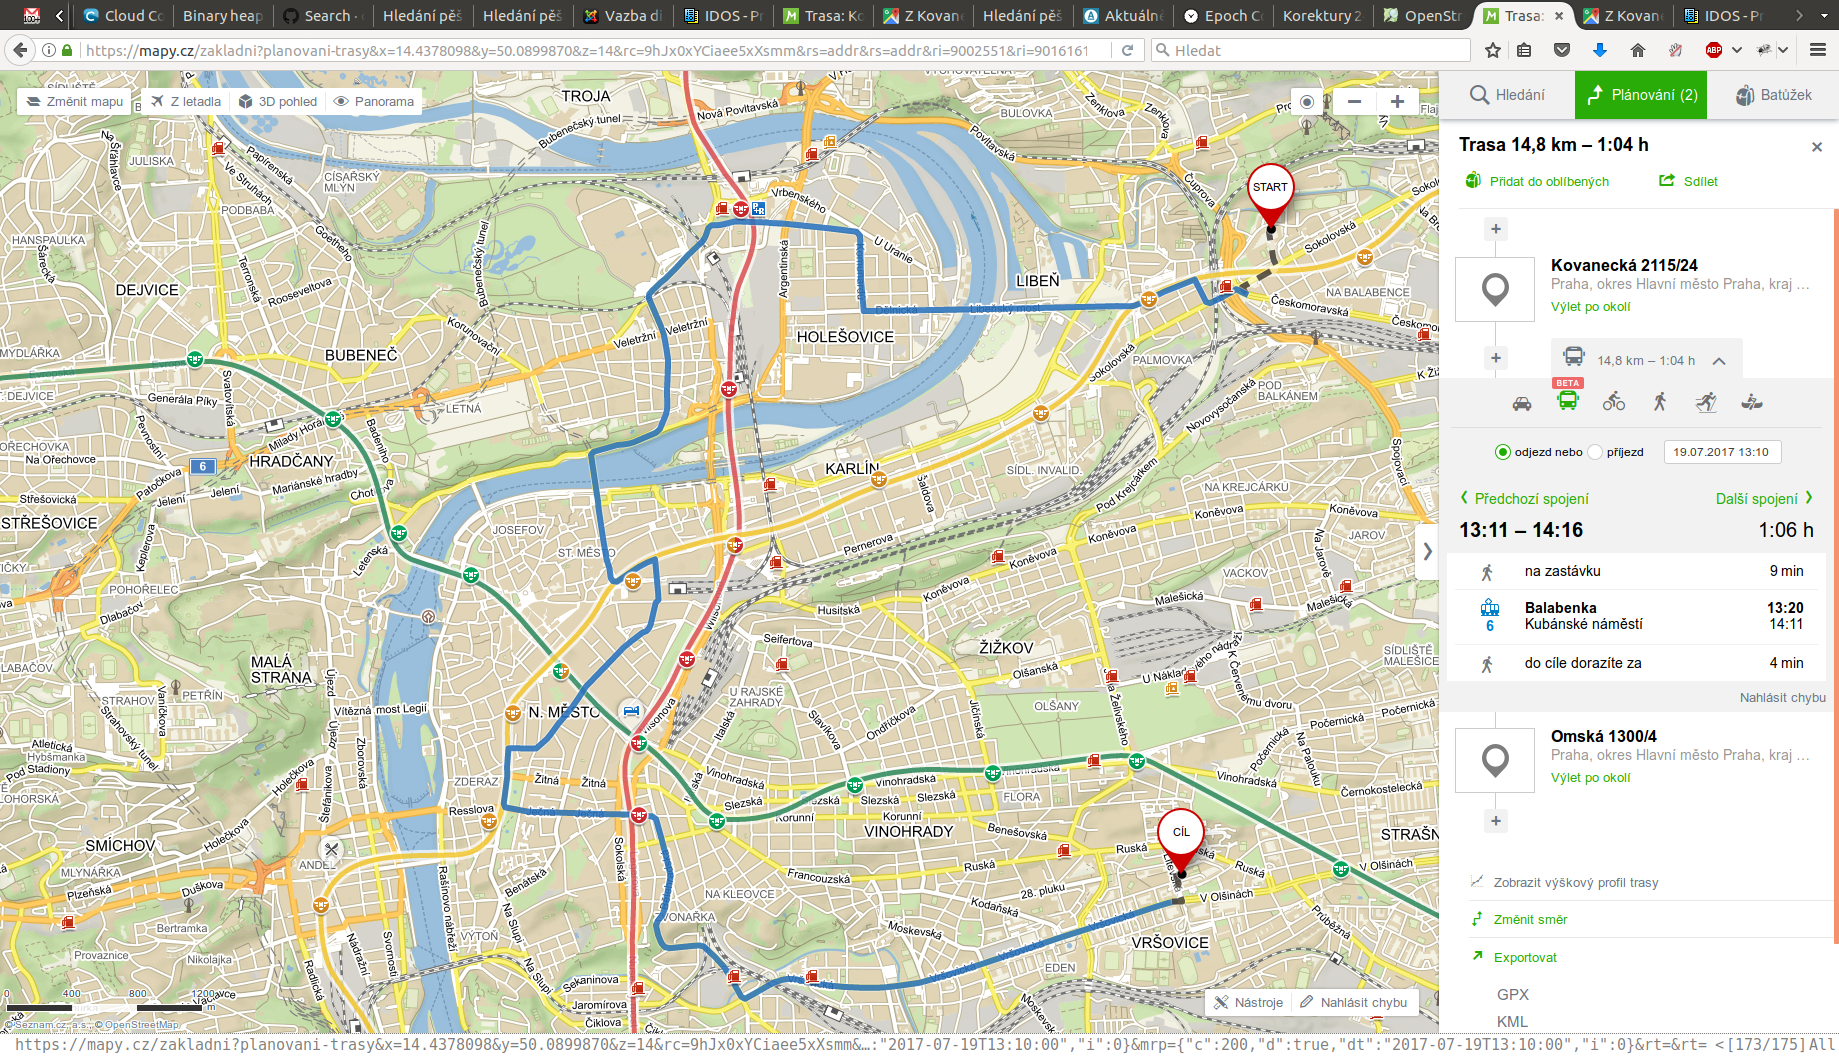
\includegraphics[width=\textwidth]{../img/kovanecka-omska-seznam.png}
  \caption{Spojení Kovanecká -- Gymnázium Omská podle Mapy.cz}
  \label{fig:kovanecka-omska-seznam}
\end{figure}
\begin{figure}[h]
  \centering
    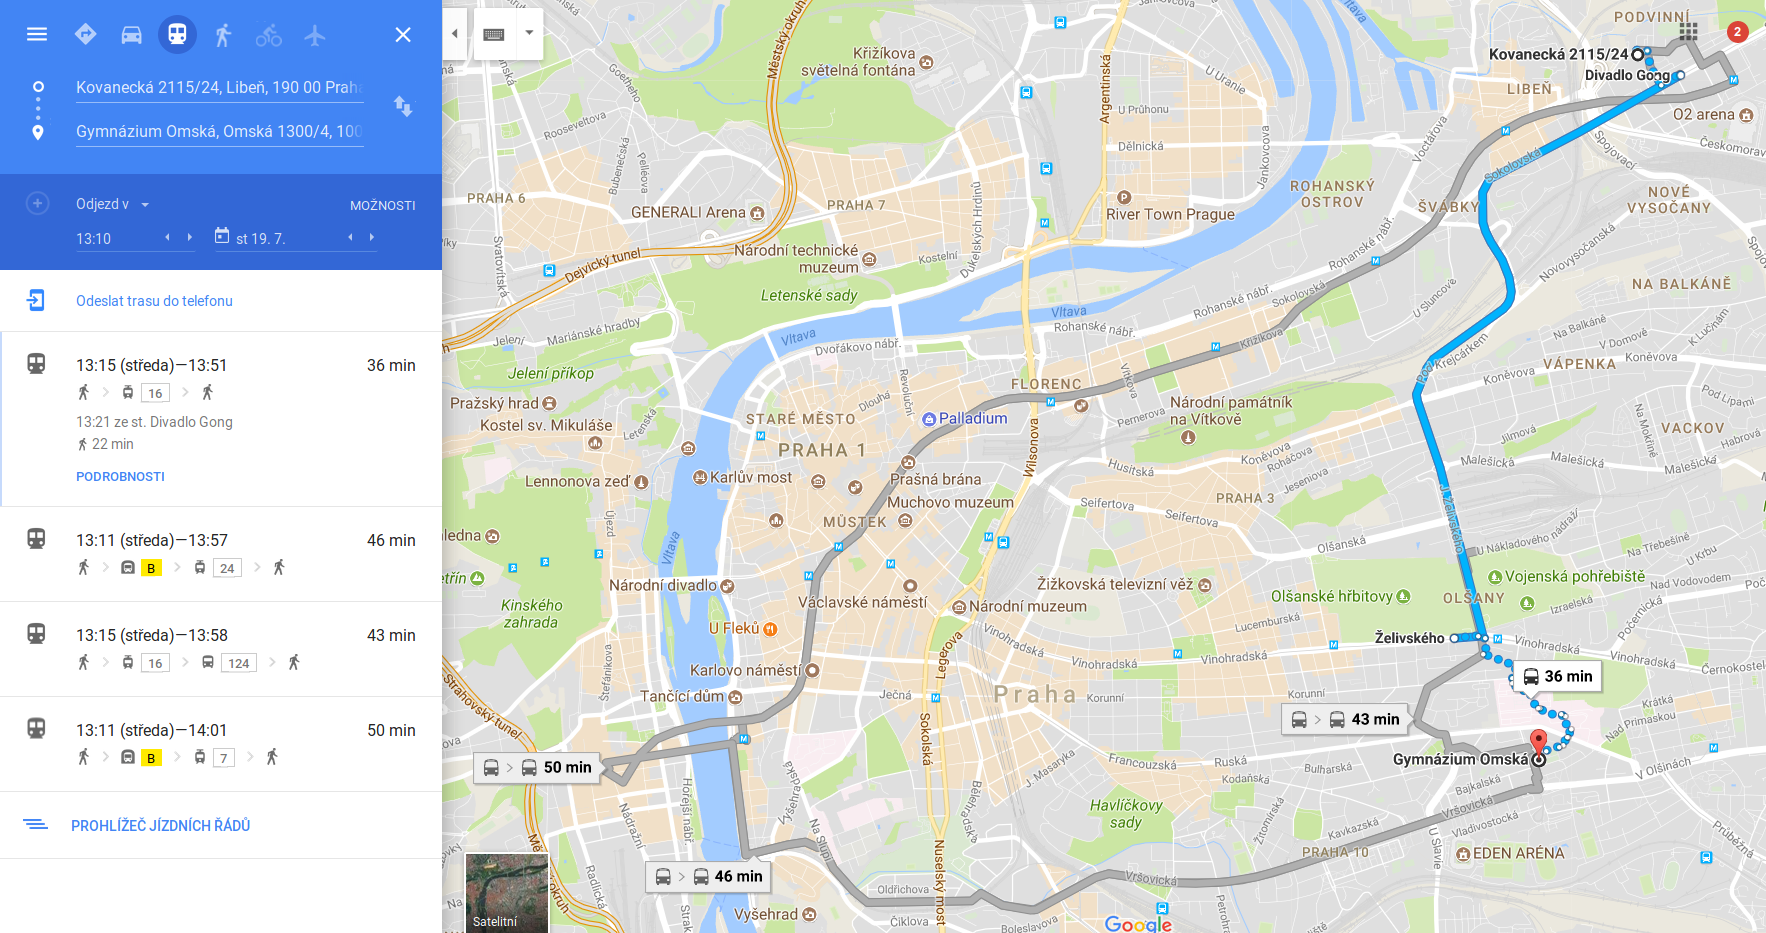
\includegraphics[width=\textwidth]{../img/kovanecka-omska-google.png}
  \caption{Spojení Kovanecká -- Gymnázium Omská podle Google Maps}
  \label{fig:kovanecka-omska-google}
\end{figure}

\clearpage
\subsection{FEL ČVUT -- Hlávkova kolej}
Spojení 0:\\[2mm]
\begin{tabular}{|l|c|c|r|}\hline
{\bf Zastávka}&{\bf Příjezd}&{\bf Odjezd}&{\bf Linka}\\\hline
Dejvická&&13:16&A\\\hline
Malostranská&13:19&13:23&2\\\hline
Moráň&13:34&&\\\hline
\end{tabular}\\[2mm]
Očekávaný příchod je 13:38.

Spojení 1:\\[2mm]
\begin{tabular}{|l|c|c|r|}\hline
{\bf Zastávka}&{\bf Příjezd}&{\bf Odjezd}&{\bf Linka}\\\hline
Lotyšská&&13:18&18\\\hline
Moráň&13:38&&\\\hline
\end{tabular}\\[2mm]
Očekávaný příchod je 13:42.


Vyhledávač IDOS našel tato spojení:\\[2mm]
\begin{tabular}{|l|c|c|r|}\hline
{\bf Zastávka}&{\bf Příjezd}&{\bf Odjezd}&{\bf Linka}\\\hline
Dejvická&&13:16&A\\\hline
Můstek&13:22&13:29&B\\\hline
Karlovo náměstí&13:32&&\\\hline
\end{tabular}\\[2mm]
\begin{tabular}{|l|c|c|r|}\hline
{\bf Zastávka}&{\bf Příjezd}&{\bf Odjezd}&{\bf Linka}\\\hline
Vítězné náměstí&&13:19&18\\\hline
Karlovo náměstí&13:37&&\\\hline
\end{tabular}\\[2mm]
\begin{tabular}{|l|c|c|r|}\hline
{\bf Zastávka}&{\bf Příjezd}&{\bf Odjezd}&{\bf Linka}\\\hline
Dejvická&&13:21&A\\\hline
Staroměstská&13:25&13:30&18\\\hline
Karlovo náměstí&13:37&&\\\hline
\end{tabular} 

Toto spojení reprezentovalo situaci, kdy samotná trasa je jednoduchá, ale je
množství různých alternativ v koncových a výchozích stanicích. Náš vyhledávač
našel spojení identická s Google Maps. Mapy.cz a IDOS nalezly mírně odlišná
spojení využívající i linku metra B, ale časově odpovídající našemu nalezenému
spojení. 

\begin{figure}[h]
  \centering
    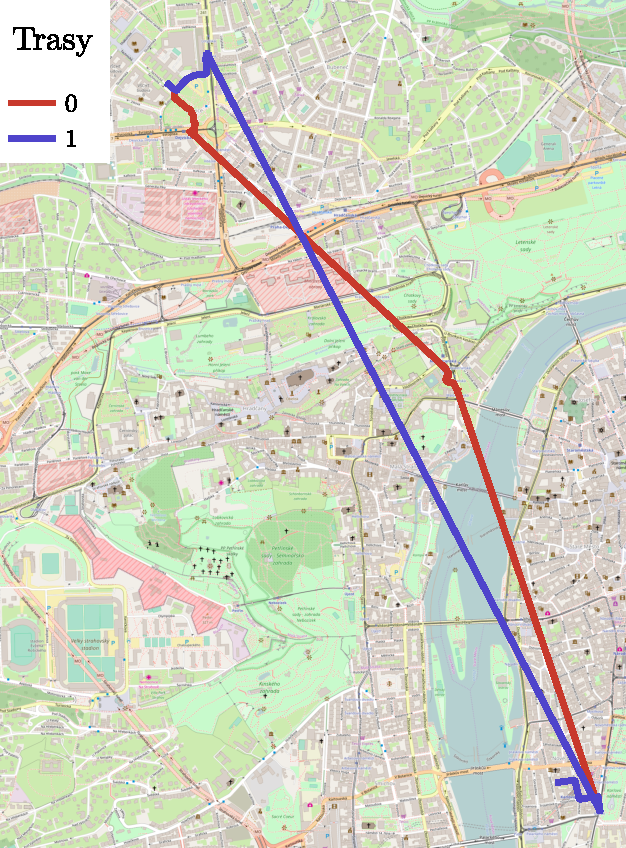
\includegraphics[width=\textwidth]{../img/fel-hlavkova-osmawalk.pdf}
  \caption{Spojení FEL ČVUT -- Hlávkova kolej podle našeho vyhledávače}
  \label{fig:fel-hlavkova-osmawalk}
\end{figure}
\begin{figure}[h]
  \centering
    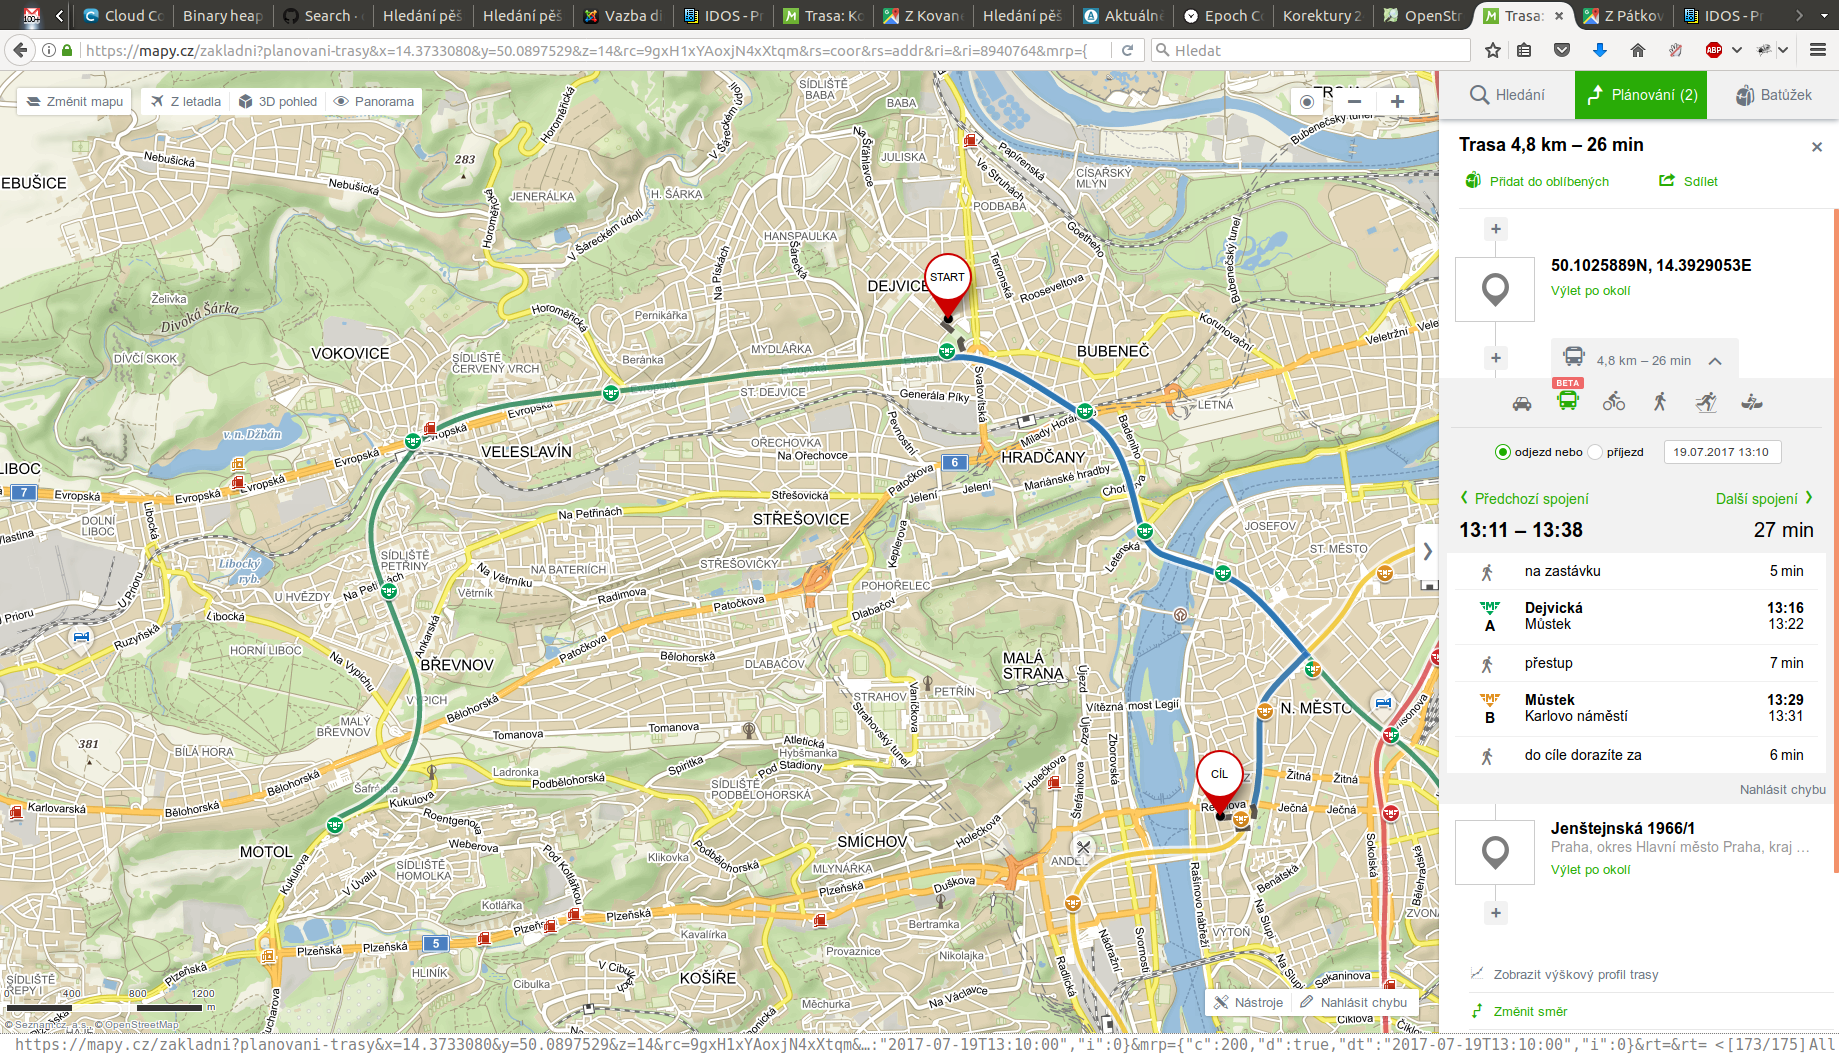
\includegraphics[width=\textwidth]{../img/fel-hlavkova-seznam.png}
  \caption{Spojení FEL ČVUT -- Hlávkova kolej podle Mapy.cz}
  \label{fig:fel-hlavkova-seznam}
\end{figure}
\begin{figure}[h]
  \centering
    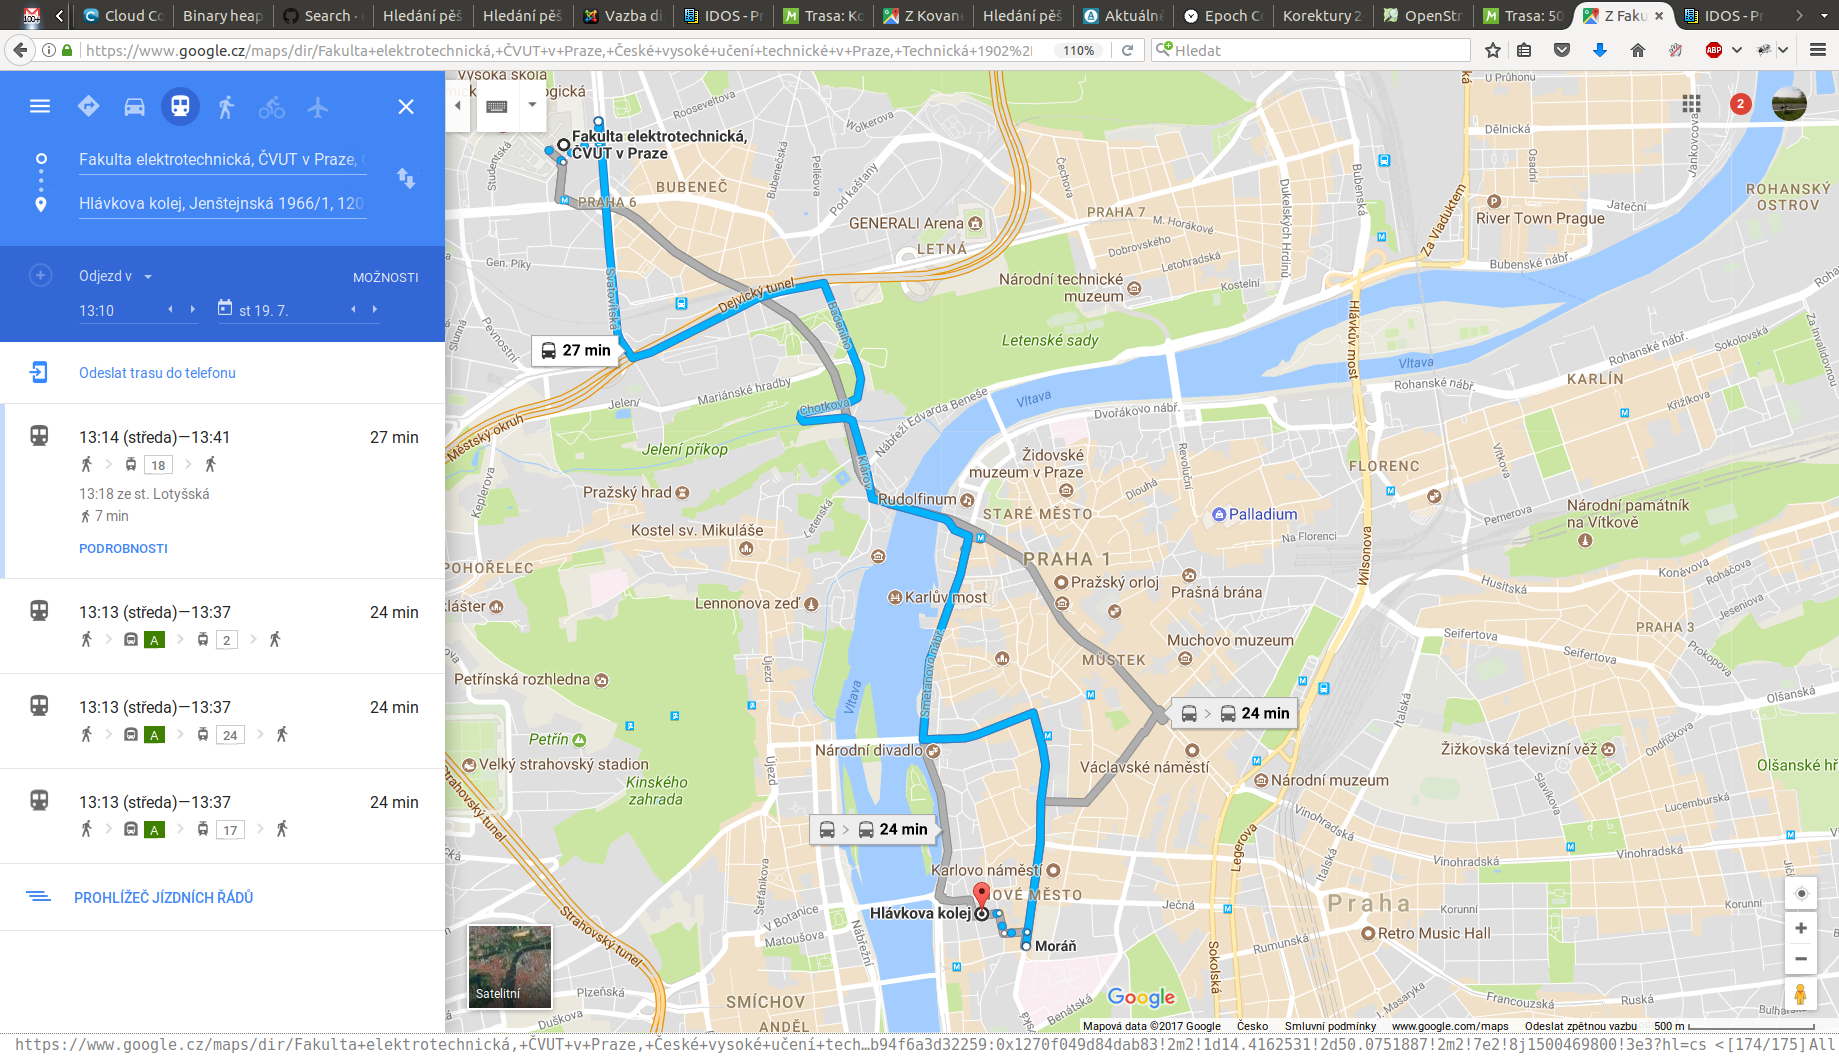
\includegraphics[width=\textwidth]{../img/fel-hlavkova-google.png}
  \caption{Spojení FEL ČVUT -- Hlávkova kolej podle Google Maps}
  \label{fig:fel-hlavkova-google}
\end{figure}

\clearpage
\section{Porovnání různých nastavení}
Pro porovnání různých nastavení našeho vyhledávače jsme zvolili trasu Kolej
17.listopadu -- Albertov, protože tato trasa poskytuje několik různých
alternativ spojení, tudíž jsme předpokládali, že se tyto alternativy projeví v
nalezených trasách. Všechna spojení byla hledána od stejného času, pracovní den
v brzkém odpoledni, tudíž by měl být eliminován vliv návazností, které fungují
jen v určité minuty, protože podmínky jsou pro všechna hledání stejné.

Porovnávali jsme tato nastavení:
\begin{itemize}
	\item {\em Standardní}\\Základní nastavení vyhledávače, měl by se chovat
	obdobně jako jiné webové vyhledávače
	\item {\em Bez autobusu 201}\\ Linka 201 je ve směru z kolejí na Nádraží
	Holešovice tak nespolehlivá, že je lepší s ní vůbec nepočítat. Toto
	nastavení ji pomocí penalty {\tt inf} vyřazuje z hledání.
	\item {\em Penalizace autobusů}\\ Test na penalizaci typu dopravního
	prostředku, měl by se snažit vyhýbat spojení autobusem a hledat jiné
	alternativy.
	\item {\em Jen jeden spoj}\\ Test na hledání, kterým spojem jet, pokud
	nechceme nikde přestupovat.
	\item {\em Pouze pěšky}\\ Ačkoli je vyhledávač stavěn na kombinované hledání
	pěších přesunů a cest MHD, stále by měl umět najít i pouze pěší cestu.
	\item {\em Na kole}\\ Tento test předpokládá jízdu na skládacím kole nebo
	koloběžce, tedy něčem, co lze vzít s sebou do MHD. Testuje nestandardní
	vyhledávací parametry.
	\item {\em Penalizace pěších přesunů}\\ Opak předchozího testu, snažíme se
	minimalizovat pěší přesuny a co nejvíce se pohybovat pomocí MHD.
\end{itemize}
\subsection{Standardní}
Nastavení je základní, takové, jaké se nachází v repozitáři jako {\tt
config/speeds.yaml}. U ostatních testů bude uveden pouze rozdíl oproti tomuto
nastavení.

Trasa nalezená vyhledávačem se standardním nastavením je již popsána výše na
obr. \ref{fig:kolej-albertov-standard}, nebudeme ji zde znovu rozebírat.
\subsection{Bez autobusu 201}
Oproti standardnímu nastavení je pouze penalizace linky 201 nastavena na {\tt
inf}, tato linka by tedy k hledání vůbec neměla být použita.

\begin{figure}[h]
  \centering
    \includegraphics{../img/kolej-albertov-bez201.pdf}
  \caption{Spojení nevyužívající autobus 201}
  \label{fig:kolej-albertov-bez201}
\end{figure}

Vyhledávač nalezl mnoho různých tras. Trasy s číslem menším než 12 mají příjezd
do 14:05, zbylé pak do 14:15. Zajímavé jsou pro nás trasy 0 a 1, protože zbylé
rychlé trasy jsou jen variacemi těchto tras. Trasa 0 odpovídá trase nalezené
standardním vylhedáváním, ale na Nádraží Holešovice využívá pěší přesun. Trasa 1
poněkud netradičně využívá přestup na linku 14 na Florenci s pěším přesunem na
Těšnov. Ve výsledcích jsou i linky, které využívají možnosti dojet na Vyšehrad a
pak sejít do nuselského údolí z druhé strany.

\subsection{Penalizace autobusů}
Oproti standardnímu nastavení mají autobusy fixní penaltu nastavenou na 100 a za
každou sekundu v autobuse dostanou penaltu dalších 10. 

\begin{figure}[h]
  \centering
    \includegraphics{../img/kolej-albertov-bus-penalta.pdf}
  \caption{Spojení penalizující autobusy}
  \label{fig:kolej-albertov-bus-penalta}
\end{figure}

Vyhledávač opět nalezl několik alternativ, které jsou velmi podobné předchozímu
vyhledávání. Je zde navíc varianta využívající dlouhý přesun tramvají č. 17 z
Trojské na Palackého náměstí a tam přestoupit do tramvaje na Albertov, která je
i podle zkušeností rychlá a spolehlivá. Všechny cesty na Trojskou a Nádraží
Holešovice v této variantě jsou pěšky z důvodu penalizace autobusů. 

\subsection{Jen jeden spoj}
Oproti standardnímu nastavení je počet nástupů do vozidla omezen na 1.

\begin{figure}[h]
  \centering
    \includegraphics{../img/kolej-albertov-jeden-spoj.pdf}
  \caption{Spojení využívající nejvýše 1 spoj MHD}
  \label{fig:kolej-albertov-jeden-spoj}
\end{figure}

Nalezené spojení je vedeno tramvají č. 17 z Trojské na Výtoň, odkud je to
na Albertov nejblíže. Cesta na Nádraží Holešovice a pak pěšky z I. P. Pavlova
byla pravděpodobně delší a proto bylo toto spojení majorizováno.

\subsection{Pouze pěšky}
Oproti standardnímu nastavení je počet nástupů do vozidla omezen na 0.
\begin{figure}[h]
  \centering
    \includegraphics{../img/kolej-albertov-pesky.pdf}
  \caption{Spojení pouze pěšky}
  \label{fig:kolej-albertov-pesky}
\end{figure}

Vyhledávač úspěšně nalezl pěší spojení až na Albertov, které by bylo
zvládnutelné, i když by to oproti cestě MHD trvalo výrazně déle. Při tomto
hledání byl vyhledávač výrazně pomalejší než pro kombinovaná spojení, což bylo
pravděpodobně způsobeno jednak mnohem větším stavovým prostorem, který bylo
potřeba projít, protože cesta trvá výrazně déle, jednak nutností zahazovat
všechna nalezená spojení pomocí MHD. Tomuto případu bychom mohli výrazně pomoci
tím, že bychom přepnuli na pouze pěší vyhledávač, ale neočekáváme, že by byly
často hledány pouze pěší trasy, proto jsme se rozhodli kód dále nerozšiřovat.

Na začátku trasy nalezl vylhedávač dvě alternativní trasy, jednu vedoucí horními
Holešovicemi přes kopec a druhou vedoucí po okraji dolních Holešovic podél
Argentinské. Ačkoli obě trasy jsou jistě zvládnutelné pěšky, ani jednu bychom si
pravděpodobně pro průchod holešovicemi nevybrali. První varianta obsahuje
zbytečné stoupání do kopce a pak klesání zpět k Vltavě, což by se dalo omezit
nastavením délkového prodloužení za kopce, problém druhé cesty, dlouhou
procházku podél čtyřproudé silnice bychom v současném stavu odstranit
nedokázali. Trasa je vedena po chodnících, tudíž penalty za silnice se
neuplatňují, bylo by potřeba při přípravě dat zjišťovat pro každou cestu objekty
v jejím bezprostředním okolí a podle toho jí přidávat atributy, na které by se
pak dal brát ohled. Toto by však bylo výpočetně náročné a je to mimo rozsah této
práce.

\subsection{Na kole}
Oproti standardnímu nastavení byly přenastaveny rychlosti pohybu na rychlosti
mezi 10 a 25 km/h (mimo schodů, kde byly nastaveny 2km/h). Rovněž byly
penalizovány cesty do kopce (10\,m délky za metr převýšení) a zvýhodňovány cesty z
kopce (-10\,m délky za metr převýšení). Navíc byla nastavena penalta za nástup
do vozidla na 100.

\begin{figure}[h]
  \centering
    \includegraphics[width=\textwidth]{../img/kolej-albertov-kolo.pdf}
  \caption{Spojení na kole}
  \label{fig:kolej-albertov-kolo}
\end{figure}

Toto vyhledávání byl spíše experiment, jak se bude vyhledávač chovat, pokud
nastavíme rychlosti výrazně výš než je obvyklá rychlost chůze. Pro vyhledávání
cyklistických tras není ve standardní konfiguraci vyhledávač vhodný, protože
klasifikuje objekty s ohledem na pěší chůzi. Pro hledání cyklistických tras by
bylo potřeba výrazně pozměnit klasifikaci objektů, zařadit například typ povrchu
silnic a pravděpodobně zahodit zkratky, protože na kole nebývají potřeba a
nemusí být tak snadno realizovatelné. V neposlední řadě existuje mnoho
kvalitních cyklistických vyhledávačů, které dávají výrazně kvalitnější výsledky
s podobnou či lepší mírou přizpůsobení, například
BRouter\footnote{\url{http://brouter.de}}.

Vyhledané trasy odpovídají očekáváním s ohledem na klasifikaci objektů. Všechny
vyhledané trasy využívají metro z Nádraží Holešovice, liší se výstupní stanicí,
kterou je buď Hlavní Nádraží, I. P. Pavlova nebo Vyšehrad. Všechny trasy by
pravděpodobně byly průjezdné, ale překvapivě se na všech trasách nachází schody,
na kterých byla nastavena rychlost na 2 km/h a tudíž se je vyplatí objet. Pro
pohodlnější cesty by bylo vhodné přidat za schody i penaltu. Ověřenou
nejrychlejší cestu z Vyšehradu, a to klesání ulicí Čiklovou a pak prokličkování
ulicí Na Slupi vyhledávač nenašel, protože v současné klasifikaci by bylo těžké
popsat vhodně rychlostní profily jednotlivých druhů komunikací a hlavně povrchů.
Dlažba na trasách vedených mimo Vyšehrad činí tyto trasy výrazně pomalejší a
velmi nepohodlné.

\subsection{Penalizace pěších přesunů}
Pěší přesun po jakémkoli typu cesty je penalizován 100 za každou sekundu
strávenou pěším přesunem.

\begin{figure}[h]
  \centering
    \includegraphics[width=\textwidth]{../img/kolej-albertov-pesi-penalty.pdf}
  \caption{Spojení penalizující pohyb pěšky}
  \label{fig:kolej-albertov-pesi-penalty}
\end{figure}

Při tomto hledání je dobře vidět princip majorizovaných tras. Je nalezena
nejrychlejší trasa, ale protože obsahuje dlouhé pěší přesuny, má vysokou
penaltu. Proto se projeví i cesty časově výrazně delší, které ale využívají více
přesunů pomocí MHD a tedy mají nížší penaltu a nejsou majorizovány. Celkem
vyhledávač nalezl čtyři základní cesty a pak další, které se však od těchto
základních liší jen drobnými detaily. Nejkratší nalezená cesta má penaltu
přibližně 86\,000, trasa 30 má penaltu nejnižší a to přibližně 12\,300. 

\section{Profilování}
Jak jsme ověřili v předchozí části, vyhledávač dává výsledky srovnatelné s
ostatními dostupnými vyhledávači spojení a má široké možnosti konfigurace.
Rychlost vyhledávání spojení je však nízká, středně dlouhá spojení přes střed
města hledá v jednotkách sekund, při specifických konfiguracích (například pouze
pěší vyhledávání) jsou ale časy výrazně delší, dosahují i desítek sekund.
Ačkoliv rychlost nebyla našim hlavním cílem, pro praktické nasazení je nezbytné,
aby vyhledávač pracoval co nejrychleji. 

Abychom zjistili, kde se při hledání tráví největší čas, profilovali jsme
vyhledávač pomocí aplikace {\tt perf}. Abychom eliminovali vliv načítání mapy a
jízdního řádu, což se při běžném vylhedávání děje jen jednou při spuštění webové
aplikace, vytvořili jsme testovací scénář pro konzolovou aplikaci. Ta si nejprve
načetla mapová data a data jízdních řádů a potom postupně hledala různá spojení
mezi předem zvolenými body. Nasbíraná data jsme pak analyzovali a na jejich
základě provedli některé optimalizace, například vyhazování majorizovaných
položek z haldy a seznamu vrcholů.

Z naměřených dat vyplývá, že místo, kde by se mělo optimalizovat nejdříve, je
cyklus porovnávající, zda právě přidávaná položka do haldy není majorizována či
naopak majorizuje nějakou jinou položku, která už v haldě je. Ve standardním
nastavení se v tomto cylku stráví okolo 25\,\% času, při hledání pouze pěších
tras je to až 50\,\%. Dalším místem v pořadí je načítání pěší hrany při
zpracovávání vrcholu a zjišťování, který její konec máme uvažovat. Zde si
myslíme, že dochází ke zpomalení převážně z důvodu přístupu na náhodné místo v
paměti, protože hran je mnoho a nejsou nijak setříděné. Překvapivě velký čas je
zabrán počítáním penalty bodu. I když se jedná o funkci obsahující pouze 2
podmínky, tráví se zde 6\,\% celkového času, což nám přišlo zvláštní, ale nemáme
pro to jasný důvod. Posledním významným časem je hledání minima v haldě, což je
ale logaritmická operace a proto nás 7\,\% stráveného času příliš nepřekvapí.


